Throughout history, mankind has always been fascinated with the physics laws governing life on Earth. The theory known as atomism was one of the first attempts to understand the nature of matter. The concept of atoms formulated by Leucippus of Abdera (5th century before the common era) and further pursued by Democritus initiated the search for the building blocks of nature~\cite{sep-atomism-ancient}. According to this theory, everything consists of "atoms" (in Greek \foreignlanguage{greek}{ἄτομος} which means uncuttable) that are physically, but not geometrically, indivisible and empty space. 

It's astounding to consider that at the turn of the twentieth century (roughly, 2500 years after atomism was formulated), the structure of the atom remained unknown. The electron had just been discovered, and its behavior and characteristics were still poorly understood. Nobody knew anything about nuclei, protons, neutrons, or other particles~\cite{intro_particle_physics}. 
Further discoveries of radioactivity (in the year 1896) and radioactive elements (in the year 1898) by H. Becquerel and M. Skłodowska-Curie marked the gateway to the 20th-century physics. 

The number of discoveries that have been made in the twentieth century is truly remarkable. Eventually, in 1970 these findings led to the formulation of a model called the Standard Model. It describes the strong, weak, and electromagnetic fundamental \footnote{the Interactions that are considered not to be reducible to more basic interactions}{interactions} between the particles. 
 High energy physics aims to explore the smallest and largest scales of the universe, seeking out new discoveries from the tiniest particles to the largest objects in space.
 
 This work aims to bring the reader on a journey from the theoretical objectives of physics, to the often complex process of development and construction of a detector for a high energy physics experiment.
 %Modern ways of conducting experiments often involve use of advanced engineering and software engineering.
 
\section{Standard Model and the strong force}

The standard model is one of the most successful theories, which to date explained numerous results from experiments worldwide. The most notably predictions of the Standard Model are the Higgs boson, W and Z bosons, the gluon, and the top and charm quark.

The standard model contains 17 particles (Figure~\ref{fig_standard})  that are the smallest building blocks and are categorized into two groups: bosons and fermions. These groups are distinguished by their quantum statistics: fermions (characterized by half-integer spin) obey Fermi–Dirac statistics and bosons (integer spin) obey Bose–Einstein statistics. 

Fermions are broken into two classes: quarks and leptons. Up and down quarks are located at the heart of atoms, inside the protons and neutrons, but the other four quarks are only observed in particle accelerator collisions.

The electron, which makes up the outer layer of atoms, is the most recognized of the leptons. Other charged leptons, known as muons and taus, are only discovered in particle accelerators and cosmic rays from space. Furthermore, each of the mentioned leptons has its corresponding neutrino, which has no electrical charge and a very small mass.

In addition to the particles, the Standard Model includes three forces that govern the behavior of matter. These forces are electromagnetism and strong and weak nuclear forces. The force particles (bosons) are the photon (electromagnetism), the gluon (strong nuclear force), the W \& Z bosons (the weak force), and the Higgs boson.

\begin{figure}[!h]
\centering
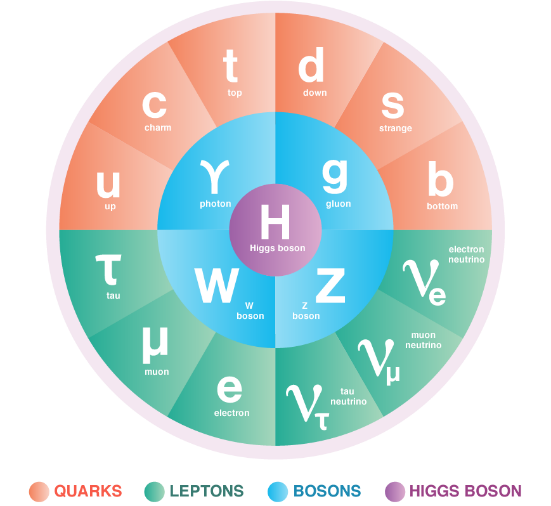
\includegraphics[width=0.65\columnwidth]{Chapter1/images/particles.png}
\caption{Fermions and bosons of the Standard Model~\cite{standard_model}.}
\label{fig_standard}
\end{figure}



The Strong Force's theoretical foundation, Quantum Chromodynamics (QCD), is well established, with quarks and gluons as the main degrees of freedom.

Yet, key phenomena in strong interactions, most notably the confinement of quarks and gluons into \footnote{Hadrons are composed of quarks, and therefore they experience the strong nuclear force}{hadrons} and the creation of mass, have remained unclear. Hot deconfined matter dominated the early cosmos just a few microseconds after the Big Bang, but compact stars may also contain cold and baryon-rich quark matter in their interiors. In extreme environments such as the high-temperature T, or the high baryon density $\rho$, the confined baryonic matter may form a new state of matter called the quark-gluon plasma (\gls{QGP})~\cite{phase_diagram}.

\section{Studying high-density matter in the laboratory}

The different phases of nuclear matter are described by the phase diagram. 

%\section{Physics goa}

